\definecolor{LightGray}{RGB}{245,245,245}
\definecolor{LightRed}{RGB}{0,0,0}
\definecolor{LightGreen}{RGB}{0,0,0}
\definecolor{LightBlue}{RGB}{100,100,100}
\lstset{ %
language=C++,                % choose the language of the code
basicstyle=\small\tt,          % print whole listing small
keywordstyle=\small\color{LightBlue},	% bold black keywords
identifierstyle=\small\color{black},           % nothing happens
commentstyle=\small\color{Rhodamine}, % white comments
stringstyle=\ttfamily,      % typewriter type for strings
showstringspaces=false,     % no special string spaces
numbers=left,                   % where to put the line-numbers
numberstyle=\tiny\tt,      % the size of the fonts that are used for the line-numbers
%stepnumber=2,                   % the step between two line-numbers. If it's 1 each line will be numbered
numbersep=5pt,                  % how far the line-numbers are from the code
%backgroundcolor=\color{LightGray},  % choose the background color. You must add \usepackage{color}
showspaces=false,               % show spaces adding particular underscores
showstringspaces=false,         % underline spaces within strings
showtabs=false,                 % show tabs within strings adding particular underscores
frame=single,			% adds a frame around the code
tabsize=3,	                % sets default tabsize to 2 spaces
%captionpos=b,                   % sets the caption-position to bottom
breaklines=true,                % sets automatic line breaking
breakatwhitespace=false,        % sets if automatic breaks should only happen at whitespace
%title={Zdrojovy kod},                 % show the filename of files included with \lstinputlisting; also try caption instead of title
%escapeinside={\%*}{*)}          % if you want to add a comment within your code
escapechar=!,
}
\chapter*{Dodatky}
\addcontentsline{toc}{chapter}{Dodatky}
\section*{Objektový model DicomPresenteru}
\addcontentsline{toc}{section}{Objektový model DicomPresenteru}
\begin{figure}
	\begin{center}
	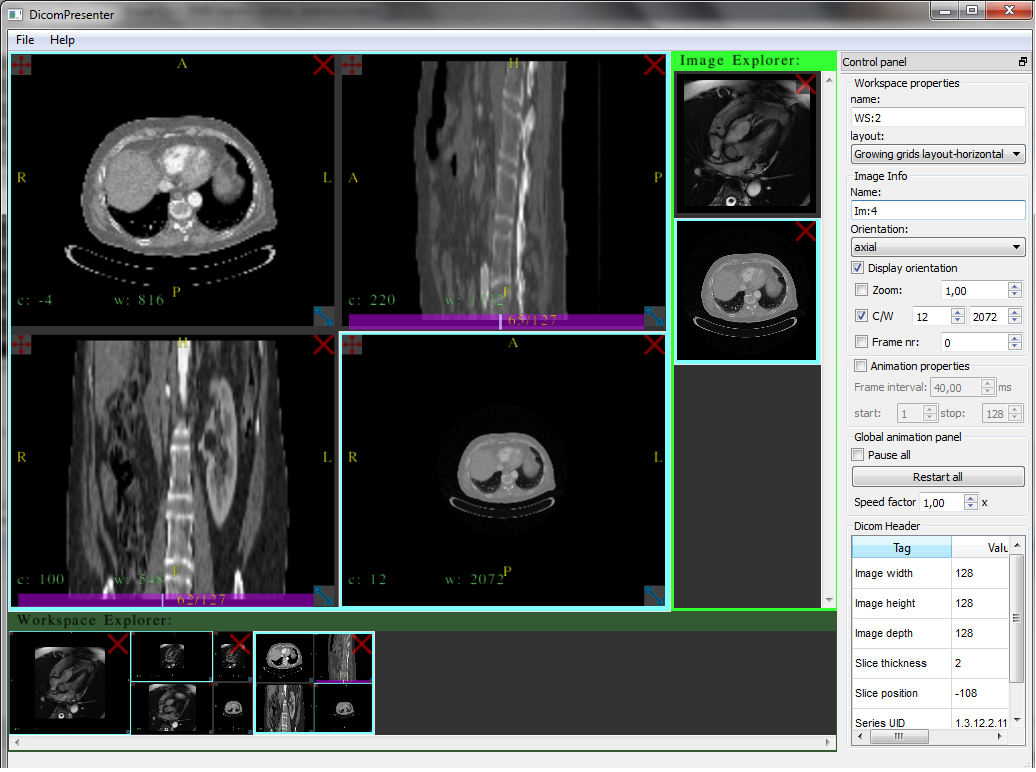
\includegraphics[width=130mm]{Text/IMG/04_GUI_Screenshot.png}
	\end{center}
	\caption{Rozhraní programu Dicom Presenter}
	\label{screenshotDP}
\end{figure}

\begin{figure}
	\begin{center}
	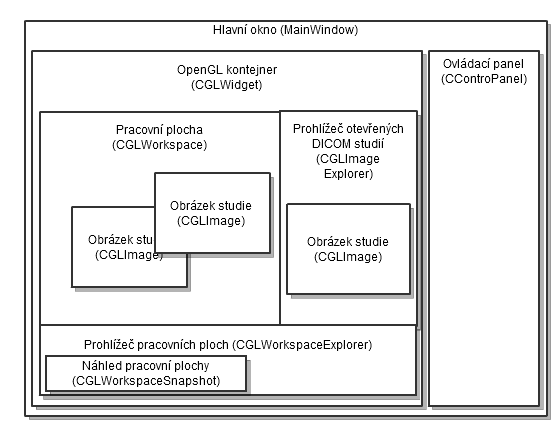
\includegraphics[width=130mm]{Text/IMG/04_GUI.png}
	\end{center}
	\caption{Reprezentace grafických prvků třídami.}
\end{figure}
\subsection*{Hlavní okno}
\addcontentsline{toc}{subsection}{Hlavní okno}

Hlavní okno programu je reprezentováno třídou \clist{Main\-Window}, která dědí třídu Qt knihovny \clist{Q\-Main\-Window}. Třída \clist{Main\-Window} obsahuje objekty tříd reprezentujících uživatelské rozhraní: \clist{CGLWidget} jež reprezentuje hlavní OpenGL okno, \clist{CControlPanel} jež představuje panel s ovládacími prvky. Oba objekty jsou zasazeny.

Třída  \clist{Main\-Window} dále vlastní objekty abstraktních tříd \clist{CDicom\-3DTexture\-Ma\-na\-ger} a \clist{CAnimation\-Manager}. Třída \clist{CDicom\-3DTexture\-Manager} pak obsahuje hashovací tabulku třídy \clist{QMap}, což je datová struktura umožňující uchování množiny dat stejného typu na základě nějakého klíče. V hashovací tabulce vlastněné třídou \clist{CDicom\-3DTexture\-Manager} jsou uloženy třírozměrné studie, každá pod unikátním řetězcem. 

Třída \clist{CAnimationManager} opět obsahuje hashovací tabulku typu \clist{QMap}, tentokrát jsou v ní uloženy informace o animacích, roli klíče plní adresa ukazatele na obrázek, pod kterým lze animaci vidět na ploše.

\subsection*{OpenGL okno}
\addcontentsline{toc}{subsection}{OpenGL okno}
Třída \clist{CGLWidget}, jež reprezentuje velké okno, do kterého jsou vykreslovány lékařské studie a některé ovládací prvky, vlastní objekty abstraktních tříd \clist{CGL\-Image\-Explorer} a \clist{CGL\-Workspace\-Explorer}.

Třída \clist{CGL\-Image\-Explorer} reprezentuje seznam otevřených studií, který je umístěn jako sloupec v pravé části okna. Třída má člen typu \clist{QList}, což je datová struktura Qt knihovny, která umožňuje uložení více prvků stejného typu pod celočíselným klíčem podobně jako pole. V této struktuře třídy \clist{CGL\-Image\-Explorer} jsou uloženy náhledy otevřených studií (třídy \clist{CGL\-Image}, viz níže).

Třída \clist{CGL\-Workspace\-Explorer} pak představuje seznam otevřených pracovních ploch, který je umístěn vespod OpenGL okna. Třída vlastní objekt typu \clist{QList}, ve kterém má uložené ukazatele na pracovní plochy (typ \clist{CGLWorkspace}). Jedna z pracovních ploch je ta, se kterou uživatel právě pracuje a vidí ji na obrazovce; ukazatel na ní je uložen ve speciální proměnné.  

\section*{Popis tříd dle funkcí}
\addcontentsline{toc}{section}{Popis tříd dle funkcí}
\subsection*{Načítání snímků}
\addcontentsline{toc}{subsection}{Načítání snímků}
Třírozměrné studie formátu DICOM jsou jsou ukládány jako série dvourozměrných obrázků s příponou \clist{.dcm}, součástí souboru je jednak hlavička s informacemi o snímku a dále připojený obrázek, nejčastěji ve formátu JPG.

Při načítání snímků do programu dochází k poměrně dlouhé sérii volání funkcí jednotlivých objektů, kterou se pokusíme popsat. Když se uživatel rozhodne načíst studii, je volána funkce \clist{main\-Window\-::Open\-File()}.  V těle funkce je pak započata série volání týkající se třídy \clist{CGL\-Image}, jejíž poslední třída volá funkci třídy \clist{Dicom3dTextureManager} a tím začíná další série volání tentokráte týkající se třídy \clist{Dicom3D\-Texture}. Po zběžném  prozkoumání se zdá být tato návaznost volání zbytečně složitá, a tak bude v příštích zásazích do programu přeskupena a pokud možno rozdělena do dvou větví. V první části je nejprve volána funkce \clist{CGL\-Image\-Explorer::Open\-Image()}, která vytváří objekt \clist{CGLImage} v jehož konstruktoru je volána funkce \clist{Dicom3d\-Texture\-Manager\-::Load\-Texture()}, ta pak vytváří objekt třídy \clist{Dicom3DTexture}. V konstruktoru poslední jmenované třídy je pak vytvoření objektu \clist{CDicomSerieData}, v jehož konstruktoru je za pomoci knihovny DCMTK načtena celá série obrázků. Třída \clist{Dicom3DTexture} pak tato data nahraje do paměti OpenGL a zachová si informace o celé studii.

\subsection*{Vybírání řezů}
\addcontentsline{toc}{subsection}{Vybírání řezů}
Po načtení studií programem, se vyplní seznam otevřených studií v pravé části OpenGL okna. Chce-li uživatel se studiemi dále pracovat, nahraje si je na pracovní plochu.

Nahrání studie na pracovní plochu lze udělat stisknutím tlačítka \clist{Add\-Image}, tím se volá funkce \clist{CControl\-Panel::\-Create\-New\-Image\-Copy()}, v jejímž těle je volána funkce \clist{CGL\-Workspace\-::Add\-Image()}. Seskupení obrázků na pracovní ploše má na starosti třída \clist{CWorkspaceLayout}, respektive pak \clist{CFree\-Layout}, nebo \clist{CGrowing\-Grid\-Layout}, a tak je volána funkce \clist{Add\-Image()} příslušné třídy.

\subsection*{Vykreslování na obrazovku}
\addcontentsline{toc}{subsection}{Vykreslování na obrazovku}
Je-li potřeba překreslit obsah OpenGL okna na obrazovku, je kdekoliv v těle programu volána funkce \clist{updateGL()}. Qt knihovna pak volá funkci \clist{CGLWidget::paintGL()}.

\subsubsection*{Funkce CGLWidget::paintGL()}
\addcontentsline{toc}{subsubsection}{Funkce CGLWidget::paintGL()}
V těle funkce \clist{CGLWidget}, která zastupuje celé OpenGL okno, pak dochází k volání funkce \clist{paintGL()} dílčích prvků a dále k volání funkcí pro vykreslení barevných ohraničení a textu.

Ve funkci \clist{CGLWidget::paintGL()} jsou nejprve volány funkce \clist{paintGL()} tříd \clist{CGLImageExplorer} a \clist{CGLWorkspaceExplorer} a dále je volána funkce \clist{paintGL()} té instance objektu typu \clist{CGLWorkspace}, která je právě aktivní:

\clist{CGLWorkspaceExplorer::GetInstance()->GetActiveWorkspace()->paintGL()}

Dále je zjištěno, zda je nějaký objekt vybrán jako aktivní a je případně volána funkce pro nakreslení barevného ohraničení:

\begin{lstlisting}[caption={Pokud je nějaký objekt aktivní je kresleno jeho barevné ohraničení.}]
if(iActiveObject) {
	iActiveObject->!\greenlist{TranslateOpenGLCoords()}!;
	iActiveObject->!\greenlist{DrawSelection()}!;
	...
}
\end{lstlisting}

Ve funkci \clist{CGLWidget::paintGL()} se dále zjišťuje, zda je aktivním objektem \clist{CGLWorkspaceExplorer} nebo \clist{CGLImageExplorer}, pak je volána funkce pro vykreslení textu.

\begin{lstlisting}[caption={Volání funkce pro vykreslení textu v případě, že aktivním objektem je \clist{CGLWorkspaceExplorer} nebo \clist{CGLImageExplorer} je realizováno operátorem \clist{dynamic\_cast}.}]
if(dynamic_cast<CGLWorkspaceExplorer*>(iActiveObject)) {
	dynamic_cast<CGLWorkspaceExplorer*>(iActiveObject)->!\greenlist{DrawTexts}!();
}

if(dynamic_cast<CGLImageExplorer*>(iActiveObject)) {
	dynamic_cast<CGLImageExplorer*>(iActiveObject)->!\greenlist{DrawTexts}!();
}
\end{lstlisting}

Zjištění, zda aktivním objektem je \clist{CGLWorkspaceExplorer} nebo \clist{CGLImageExplorer} je realizováno operátorem \clist{dynamic\_cast}.

Operátor \clist{dynamic\_cast<A*>(B)} vrací ukazatel typu A* na objekt B. Zaručuje tak v našem případě, že vraceným ukazatelem nebude \clist{CGLObject*}, ale \clist{CGLWorkspaceExplorer*} nebo \clist{CGLImageExplorer*}.

\subsubsection*{Funkce CGLImageExplorer::paintGL() a CGLWorkspaceExplorer::paintGL()}
\addcontentsline{toc}{subsubsection}{Funkce CGLImageExplorer::paintGL() a CGLWorkspaceExplorer::paintGL()}
Ve funkci \clist{CGLImageExplorer::paintGL()}, je vytvořen iterátor všech obrázků jež spravuje \clist{CGLImageExplorer}. Dále jsou volány funkce \clist{paintGL()} všech obrázků, jež se vejdou na pracovní plochu (tato podmínka však byla z příkladu vypuštěna):

\begin{lstlisting}[caption={Volání funkce \clist{paintGL()} studií, jež spravuje \clist{CGLImageExplorer}.}]
QListIterator<CGLImage*> images(iImages);
while (images.hasNext()){
	CGLImage *im = images.next();
	...
	im->paintGL();
}
\end{lstlisting}


Ve funkci \clist{CGLWorkspaceExplorer::paintGL()} je opět podobným způsobem jako v případě \clist{CGLImageExplorer} vytvořen iterátor a volány funkce \clist{paintGL()} jednotlivých objektů, které třída spravuje (tentokrát pracovní plochy), tím je vykreslen seznam pracovních ploch.

\subsubsection*{Funkce  CGLWorkspace::paintGL()}
\addcontentsline{toc}{subsubsection}{Funkce  CGLWorkspace::paintGL()}
Při volání

\clist{CGLWorkspaceExplorer::GetInstance()->GetActiveWorkspace()->paintGL()}

\noindent je volána funkce pro vykreslení viditelné pracovní plochy, se kterou uživatel právě pracuje. V této funkci je volána dvojice funkcí: \clist{CGLWorkspace\-::Draw\-To\-Texture()} a \clist{CGL\-Workspace\-::Draw\-From\-Texture()}. V první funkci je vykreslen celý obsah pracovní plochy do textury, ve druhé je pak tato textura vykreslena na obrazovku (na své místo mezi seznam obrázků a seznam pracovních ploch)

Ve funkci \clist{CGL\-Workspace::\-Draw\-To\-Texture()} je nejprve aktivován frame-buffer Qt knihovny pro vykreslování do textury. Dále je vytvořen iterátor prvků \clist{CGLImage} a postupně jsou všechny obrázky vykreslovány na obrazovku.
 

\subsection*{Manipulace se snímky}
\addcontentsline{toc}{subsubsection}{Manipulace se snímky}
Třírozměrné studie jsou za běhu programu načteny v OpenGL paměti, v pravé části okna v seznamu otevřených studií je vidět vždy náhled na danou studii. Studie se kterými uživatel pracuje, jsou pak vyobrazeny v nějakém svém řezu na pracovní ploše. Program prozatím nabízí zobrazení studií v řezu podle jedné z hlavních rovin (čelní, předozadní a příčné).

Řez na pracovní ploše je reprezentován třídou \clist{CGL\-Image}. V konstruktoru třídy je volána funkce \clist{CGL\-Image\-::Draw\-Slice\-From\-3D\-Texture\-To\-Actual\-Slice\-Texture()}, ve které je do frame-bufferu vykreslen řez třírozměrnou studií. Pokud pak za běhu programu chce uživatel se studií manipulovat, jsou uživatelské akce (pohyby myši) zaznamenávány třídou \clist{CGLWidget} a předávány objektu třídy \clist{CGLImage}, který je právě vybrán jako aktivní. Jedná se o akce Qt knihovny \clist{mouse\-Move\-Event, wheel\-Event}. Ve funkci \clist{CGL\-Image::\-mouse\-Move\-Event()} jsou pak tyto akce analyzovány a jsou volány příslušné funkce. V případě, že se jedná pouze o zvětšení, či přemístění výřezu na pracovní ploše, není třeba znovu číst třírozměrnou texturu a jsou volány funkce \clist{Set\-Zoom(), Set\-Geometry()} a následně funkce Qt knihovny \clist{update\-GL()}. Pokud se jedná o posuv řezu v rámci třírozměrné textury, je započata série volání: \clist{Move\-ToFrame()}, \clist{Move\-ToDepth()} a opět se volá funkce \clist{Draw\-Slice\-From\-3DTexture\-To\-Actual\-Slice\-Texture()}. V poslední jmenované funkci je vykreslen adekvátní řez třírozměrnou studií, který odpovídá posunutí. Ve funkci jsou dále volány příkazy pro výpočet pixel shader skriptu na grafické kartě.

\subsection*{Export pracovní plochy a videa}
\addcontentsline{toc}{subsubsection}{Export pracovní plochy a videa}
Export pracovní plochy je realizován funkcí \clist{Main\-Window::Save\-Snapshot()}, kde je volána funkce \clist{CGL\-Workspace\-::Save\-Texture()} a dále funkce \clist{CGL\-Workspace\-::Draw\-To\-Texture()}.

Práci na ploše lze zachytit, ale jen s využitím externího programu, čímž se funkce omezuje jen na OS Windows. Informace o animaci (délka, počet snímků) jsou uloženy v objektu třídy \clist{CAnimation}.


\subsection*{Abstraktní třída CGLObject}
\addcontentsline{toc}{subsubsection}{Abstraktní třída CGLObject}
Třídy jež reprezentují objekty na pracovní ploše jsou \clist{CGLWidget}, \clist{CGLImageExplorer}, \clist{CGLImage}, \clist{CGLWorkspaceExplorer}, \clist{CGLWorkspace}, \clist{CGLWorkspaceSnapshot}. Jejich společné vlastnosti jsou seskupeny ve třídě \clist{CGLObject}, jež všechny jmenované objekty dědí. Mezi společné vlastnosti patří: přepočet souřadnic z Qt na OpenGL, vykreslování barevného ohraničení objektu, vykreslování ikonek.

Při takovém zobecnění lze psát kód:

\begin{lstlisting}[caption={Zobecnění pomocí abstraktní funkce \clist{CGLObject}.}]
!\greenlist{CGLObject}! *iActiveObject;
...
if (...) iActiveObject = !\greenlist{iWorkspaceExplorer}!;
if (...) iActiveObject = !\greenlist{CGLWorkspaceExplorer::GetInstance()->GetActiveWorkspace()}!;
...
iActiveObject->!\greenlist{DrawSelection()}!;
\end{lstlisting}

V příkladu je deklarován ukazatel na objekt typu \clist{CGLObject}, což díky zobecnění může být objekt typu \clist{CGLWorkspaceExplorer}, \clist{CGLWorkspace} apod. Během používání programu je uložena do ukazatele adresa objektu, se kterým uživatel právě pracuje.

Když dochází k překreslení pracovní plochy a je třeba nakreslit zvýrazněné hranice kolem aktivního objektu, je možné volat funkci \clist{iActive\-Object\-->Draw\-Selection\-()}, aniž bychom museli znát, zda aktivním objektem je pracovní plocha, prohlížeč pracovních ploch, nebo nějaký obrázek.



